\documentclass[12pt,letterpaper]{article}

\usepackage[spanish]{babel}
\usepackage[utf8]{inputenc}
\usepackage[T1]{fontenc}
\usepackage{amsmath,amssymb,amsfonts}
\usepackage{graphicx}
\usepackage{textcomp}
\usepackage{xcolor}
\usepackage[margin=2.5cm]{geometry}
\usepackage{booktabs}
\usepackage{longtable}
\usepackage{array}
\usepackage{tikz}
\usepackage{fancyhdr}
\usepackage{listings}
\usepackage{hyperref}
\usepackage{enumitem}
\usetikzlibrary{positioning,arrows.meta,shapes.geometric}

\hypersetup{
  colorlinks=true,
  linkcolor=black,
  citecolor=black,
  urlcolor=blue,
  pdftitle={Localización del LCA en RM de rodilla: preparación de los datos},
  pdfauthor={Christopher Zúñiga}
}

\pagestyle{fancy}
\fancyhf{}
\fancyhead[L]{CI-0148 Aprendizaje Automático}
\fancyhead[R]{Entregable 2 --- CRISP-ML(Q), fase 2}
\fancyfoot[C]{\thepage}
\setlength{\headheight}{15pt}

\definecolor{codebg}{HTML}{F6F6F4}
\definecolor{codecomment}{HTML}{6B6A63}
\definecolor{codekw}{HTML}{1C5CAB}
\definecolor{codestr}{HTML}{A8481F}
\lstset{
  language=Python,
  basicstyle=\ttfamily\footnotesize,
  keywordstyle=\color{codekw}\bfseries,
  commentstyle=\color{codecomment}\itshape,
  stringstyle=\color{codestr},
  backgroundcolor=\color{codebg},
  frame=single,
  rulecolor=\color{codebg},
  breaklines=true,
  columns=fullflexible,
  keepspaces=true,
  showstringspaces=false,
  numbers=left,
  numberstyle=\tiny\color{codecomment},
  xleftmargin=1.5em,
  framexleftmargin=1.5em,
  captionpos=b
}
\renewcommand{\lstlistingname}{Código}
\renewcommand{\lstlistlistingname}{Índice de código}

\newcommand{\code}[1]{\texttt{\hyphenchar\font=-1 #1}}
\emergencystretch=2em

\title{
  Localización del ligamento cruzado anterior en resonancias magnéticas de rodilla\\[0.3em]
  \large Entregable 2: Preparación de los datos (CRISP-ML(Q), fase 2)
}
\author{Christopher Zúñiga, C28730 \\ \small Escuela de Ciencias de la Computación e Informática \\ \small Universidad de Costa Rica --- CI-0148 Aprendizaje Automático}
\date{Octubre de 2026}

\begin{document}

\maketitle

\begin{abstract}
\noindent
Este documento corresponde al segundo entregable del curso CI-0148 y desarrolla la fase 2 de CRISP-ML(Q): preparación de los datos. A partir del planteamiento de la fase 1 ---localizar el ligamento cruzado anterior (LCA) en volúmenes de resonancia magnética (RM) del conjunto KneeMRI---, se construyó un pipeline reproducible que (i) inventaria y verifica los 917 volúmenes del conjunto, (ii) aplica una puerta de calidad automatizada que detiene el proceso ante cualquier inconsistencia, (iii) particiona los datos en un conjunto de prueba reservado y cinco pliegues de validación cruzada, agrupando por examen y estratificando por diagnóstico, antes de cualquier transformación, (iv) normaliza la intensidad por volumen y uniformiza el tamaño en plano sin alterar las coordenadas de la caja objetivo, y (v) genera un índice de 28\,359 cortes para un modelo de aprendizaje profundo 2.5D. Se documenta además la estrategia para los dos desbalances del problema (cortes con y sin LCA, y severidad del diagnóstico). Todas las verificaciones de calidad pasaron: ningún examen aparece en más de una partición y la proporción de clases de cada partición se desvía como máximo 0.54 puntos porcentuales del total. El pipeline se acompaña de 31 pruebas unitarias y de documentación para reconstruir el conjunto. El documento cierra con una revisión honesta del plan: el entregable llega a tiempo según el calendario vigente del curso, pero el proyecto va unos diez días atrás respecto a su propio plan.
\end{abstract}

\vspace{0.5em}
\noindent\textbf{Palabras clave:} preparación de datos, fuga de información, validación cruzada agrupada, desbalance de clases, resonancia magnética, CRISP-ML(Q).

\vspace{1em}
\tableofcontents
\thispagestyle{fancy}

\newpage
% =========================================================================
\section{Introducción}
% =========================================================================

En la fase 1 de este proyecto se planteó una tarea de aprendizaje automático orientada a apoyar la lectura clínica de resonancias magnéticas de rodilla: \textbf{localizar automáticamente el ligamento cruzado anterior (LCA)} dentro del volumen, es decir, predecir la caja delimitadora tridimensional que lo contiene. El LCA es una banda delgada y oblicua que aparece en apenas unos pocos cortes sagitales consecutivos; un especialista debe encontrarla antes de poder evaluar si está sana, parcialmente lesionada o rota. Automatizar ese primer paso de ubicación permite que el radiólogo, o un modelo posterior de clasificación, concentre su atención en la región correcta.

El conjunto de datos es KneeMRI \cite{stajduhar2017semi,zenodo_kneemri}: 917 resonancias de rodilla vistas de lado (cortes sagitales), con una configuración que oscurece la grasa para que ligamentos y líquido resalten mejor, adquiridas en un único equipo Siemens Avanto 1.5\,T del Clinical Hospital Centre Rijeka (Croacia) entre 2006 y 2014. Cada examen trae un diagnóstico de severidad (\code{aclDiagnosis}: 0 sano, 1 parcial, 2 roto) y una caja delimitadora 3D alrededor del LCA trazada manualmente por los autores. En la fase 1 se estableció como línea base una caja fija promedio, que alcanza un IoU medio de 0.391, y se fijó como criterio de éxito un IoU medio de al menos 0.5 en el conjunto de prueba.

\paragraph{Contexto de la preparación de datos.} En CRISP-ML(Q) \cite{studer2021crispmlq}, la preparación de datos es la fase que transforma los datos crudos en un conjunto listo para entrenar, y suele ser la que más tiempo consume. El modelo de proceso exige, además, que cada tarea tenga un método de aseguramiento de calidad (Q) con un criterio verificable. Para este proyecto, el contexto impone tres riesgos concretos:

\begin{enumerate}[leftmargin=*]
  \item \textbf{Fuga de información} \cite{kaufman2012leakage}. Algunos exámenes tienen varias series de la misma rodilla; si una serie cae en entrenamiento y otra en prueba, el modelo se evalúa sobre una rodilla que ya vio. Del mismo modo, cualquier estadística calculada con todos los datos antes de particionar filtra información del conjunto de prueba al entrenamiento.
  \item \textbf{Desbalance}. El diagnóstico está desbalanceado (75.2\,\% sanos, 18.8\,\% parciales, 6.0\,\% rotos), y, como el LCA ocupa solo de 2 a 6 de los 21 a 45 cortes de cada volumen, alrededor de nueve de cada diez cortes no contienen el ligamento.
  \item \textbf{Transformaciones irreproducibles}. En imágenes médicas abundan decisiones (tamaño, normalización, orientación) que, si se aplican de forma manual o en cuadernos ejecutados en desorden, no pueden reconstruirse ni auditarse.
\end{enumerate}

\noindent Entre la fase 1 y esta fase se tomó además una decisión que condiciona todo el preprocesamiento: el modelado se hará con \textbf{aprendizaje profundo sobre una representación 2.5D} (cada corte se acompaña de sus dos vecinos), en lugar de un modelo clásico con características diseñadas a mano o de una red 3D sobre el volumen completo. La justificación se presenta en la Sección~\ref{sec:transformaciones}.

\paragraph{Organización del documento.} La Sección~\ref{sec:metodos} (Materiales y métodos) lista los recursos y herramientas utilizados y describe, con su justificación y muestras de código, cada etapa del pipeline: inventario, puerta de calidad, partición, transformaciones, índice de cortes, estrategia de desbalance y reproducibilidad. La Sección~\ref{sec:discusion} analiza los resultados obtenidos y los contrasta con los criterios de calidad definidos en la fase 1. La Sección~\ref{sec:plan} revisa el avance frente al plan de la propuesta, y la Sección~\ref{sec:conclusiones} presenta las conclusiones.

% =========================================================================
\section{Materiales y métodos}\label{sec:metodos}
% =========================================================================

\subsection{Recursos utilizados}

\paragraph{Datos.} Se usó la versión completa de KneeMRI publicada en Zenodo \cite{zenodo_kneemri} (917 archivos \code{.pck} con arreglos NumPy \code{uint16}, 6.2\,GB, licencia CC BY-NC-ND 4.0) junto con el archivo \code{metadata.csv} de la redistribución de Kaggle \cite{kaggle_kneemri}. La razón de usar dos fuentes se explica en la Sección~\ref{sec:manifiesto}.

\paragraph{Poder computacional.} Todo el trabajo se ejecutó en una computadora portátil personal: procesador Apple M1 (8 núcleos), 16\,GB de memoria unificada y macOS 26.6. El pipeline completo no requiere GPU y se ejecuta en unos 67\,s, de los cuales 51\,s corresponden al procesamiento de los volúmenes.

\paragraph{Software.} Python 3.14.4 en un entorno virtual con dependencias fijadas en \code{requirements.txt}: NumPy 2.5.2 \cite{harris2020numpy}, pandas 3.0.5 \cite{mckinney2010pandas}, scikit-learn 1.9.1 \cite{pedregosa2011sklearn}, SciPy 1.18.1, PyYAML 6.0.3, Matplotlib 3.11.1 y pytest 9.1.1.

\paragraph{Recursos humanos.} Un único estudiante. No se contó con un especialista clínico para revisar las anotaciones; esta limitación ya se había declarado en la fase 1 y se retoma en la Sección~\ref{sec:discusion}. Como apoyo se usó un asistente de programación basado en IA para revisar código y discutir decisiones de diseño; las decisiones y la implementación son del autor.

\paragraph{Referentes metodológicos.} La organización del proyecto sigue la convención de Cookiecutter Data Science \cite{cookiecutter_ds} (datos crudos inmutables, datos intermedios y procesados regenerables). Las decisiones de normalización siguen las de nnU-Net \cite{isensee2021nnunet}, la referencia de facto para el preprocesamiento de imágenes médicas, y la representación por cortes sigue la práctica de MRNet \cite{bien2018mrnet}, el antecedente más citado de aprendizaje profundo en RM de rodilla.

\subsection{Arquitectura del pipeline}

La Figura~\ref{fig:pipeline} resume el flujo. El pipeline se rige por cuatro principios:

\begin{enumerate}[leftmargin=*]
  \item \textbf{Los datos crudos no se modifican nunca}. Todo lo que se genera vive en \code{datasets/interim/} y \code{datasets/processed/}, y puede borrarse y regenerarse.
  \item \textbf{La lógica vive en funciones puras} dentro de \code{src/data/}: reciben datos y devuelven datos, sin leer configuración ni escribir archivos. Esto las hace probables de forma aislada y reutilizables en la fase 3.
  \item \textbf{Un único punto de entrada}, \code{scripts/build\_dataset.py}, lee la configuración, ejecuta las etapas en orden y escribe los resultados. Los cuadernos de Jupyter se usan solo para exploración y nunca producen artefactos de los que dependa el pipeline.
  \item \textbf{Toda decisión está en la configuración} (\code{configs/prep.yaml}, Código~\ref{lst:config}), incluida la semilla aleatoria; ningún parámetro está escrito directamente en el código.
\end{enumerate}

\begin{figure}[!htbp]
\centering
\begin{tikzpicture}[
  node distance=0.45cm and 0.5cm,
  pstep/.style={draw=black!60, rounded corners=3pt, fill=black!4, align=center, font=\footnotesize, minimum height=1.05cm, text width=2.2cm},
  pdata/.style={draw=black!40, dashed, rounded corners=3pt, align=center, font=\scriptsize\ttfamily, text width=2.2cm},
  pgate/.style={pstep, fill=orange!12, draw=orange!60!black},
  arr/.style={-{Stealth[length=2mm]}, black!60}
]
\node[pdata] (raw) {metadata.csv\\917 .pck};
\node[pstep, right=of raw] (man) {1. Manifiesto\\\scriptsize inventario y forma};
\node[pgate, right=of man] (qa) {2. Puerta de\\calidad (Q)};
\node[pstep, right=0.9cm of qa] (split) {3. Partición\\\scriptsize SGKF agrupada};
\node[pstep, below=0.9cm of split] (tr) {4. Transformar\\\scriptsize recorte, z, padding};
\node[pstep, left=of tr] (idx) {5. Índice de\\cortes 2.5D};
\node[pdata, left=of idx] (out) {volumes/*.npy\\slices.csv};

\node[pdata, below=0.35cm of man] (o1) {manifest.csv};
\node[pdata, below=0.35cm of qa] (o2) {qa\_report.csv};
\node[pdata, right=0.35cm of split, text width=1.6cm] (o3) {splits.csv};

\draw[arr] (raw) -- (man);
\draw[arr] (man) -- (qa);
\draw[arr] (qa) -- node[above, font=\tiny]{pasa} (split);
\draw[arr] (split) -- (tr);
\draw[arr] (tr) -- (idx);
\draw[arr] (idx) -- (out);
\draw[arr, dotted] (man) -- (o1);
\draw[arr, dotted] (qa) -- (o2);
\draw[arr, dotted] (split) -- (o3);
\end{tikzpicture}
\caption{Pipeline de preparación de datos. Cada etapa es una función pura en \code{src/data/}; \code{scripts/build\_dataset.py} las encadena y guarda los artefactos (recuadros punteados). Si la puerta de calidad encuentra cualquier problema, el pipeline se detiene antes de particionar.}
\label{fig:pipeline}
\end{figure}

\begin{lstlisting}[language={}, caption={Configuración completa del pipeline (\code{configs/prep.yaml}).}, label={lst:config}]
seed: 42
data:
  metadata_csv: datasets/raw/kneemridataset/metadata.csv
  volumes_dir: datasets/raw/volumetric_data
  interim_dir: datasets/interim
  processed_dir: datasets/processed
preprocess:
  clip_low_pct: 0.5
  clip_high_pct: 99.5
  pad_height: 320
  pad_width: 320
  storage_dtype: float16
split:
  n_test_splits: 6
  n_cv_folds: 5
  max_prop_diff: 0.02
\end{lstlisting}

\subsection{Manifiesto: inventario verificado de los datos}\label{sec:manifiesto}

El primer paso construye un \emph{manifiesto}: una tabla con una fila por volumen que reúne los metadatos del conjunto con información verificada directamente sobre los archivos (ruta, existencia, forma, tipo de dato e intensidades mínima y máxima). Todas las etapas posteriores leen esta tabla en lugar de recorrer carpetas, de modo que no puedan discrepar sobre qué volúmenes existen.

\paragraph{Datos faltantes.} Al construir el primer manifiesto sobre la descarga de Kaggle se confirmó el hallazgo de la fase 1: solo 736 de los 917 archivos existían (faltaban las carpetas \code{vol09} y \code{vol10}), y entre los faltantes había 10 de los 55 casos de rotura completa. Como perder el 18\,\% de la clase más escasa comprometía la estratificación, se descargó el conjunto completo desde Zenodo \cite{zenodo_kneemri}. Antes de usarlo se verificó que (i) los 917 nombres de \code{metadata.csv} tienen archivo correspondiente, sin archivos sobrantes, y (ii) los 736 archivos comunes a ambas fuentes son idénticos byte a byte (mismo hash MD5). Esto permite combinar el \code{metadata.csv} de Kaggle con los volúmenes de Zenodo sin ambigüedad.

\paragraph{Clave primaria.} \code{examId} no es único: 7 exámenes tienen más de una serie (seis con dos y uno con tres), de modo que los 917 volúmenes corresponden a 909 exámenes. La clave es el par (\code{examId}, \code{seriesNo}), y el manifiesto falla de inmediato si encuentra un par duplicado, antes de abrir ningún archivo. Las rutas se guardan relativas a la carpeta de volúmenes, de modo que el manifiesto es portable entre máquinas.

\subsection{Puerta de calidad}

Antes de particionar, la función \code{run\_qa\_checks} evalúa el manifiesto con reglas fijas (Tabla~\ref{tab:qa}). En lugar de detenerse en el primer error, recoge todos los problemas en un reporte (\code{qa\_report.csv}) que se guarda siempre; si el reporte no está vacío, el pipeline se detiene. Un reporte vacío, con solo encabezados, es la evidencia de que la verificación se ejecutó y pasó. Como las reglas no aprenden nada de los datos, ejecutarlas sobre el conjunto completo no introduce fuga.

\begin{table}[!htbp]
\centering
\small
\caption{Verificaciones de la puerta de calidad y su justificación.}
\label{tab:qa}
\begin{tabular}{p{3.2cm}p{5.3cm}p{5.6cm}}
\toprule
Verificación & Regla & Por qué importa \\
\midrule
Etiquetas válidas & \code{aclDiagnosis} $\in\{0,1,2\}$, \code{kneeLR} $\in\{0,1\}$ & Un valor inválido crearía una cuarta ``clase'' en la estratificación. \\
Archivo presente & existe el \code{.pck} de cada fila & Un volumen faltante cambiaría la partición en silencio. \\
Tamaño de la caja & ancho, alto y profundidad $>0$ & Una caja vacía no es un objetivo aprendible. \\
Caja dentro del volumen & en cada eje: inicio $\geq 0$ e inicio $+$ tamaño $\leq$ dimensión & La caja es la variable objetivo; si sale del volumen no puede aprenderse ni recortarse. \\
Tipo de dato & \code{uint16} en todos los volúmenes & La normalización asume enteros de 12 bits. \\
Intensidad & máximo $>0$ y $\leq 4095$ & Detecta volúmenes vacíos o fuera del rango de 12 bits. \\
\bottomrule
\end{tabular}
\end{table}

\noindent La verificación de límites no puede detectar si los ejes $x$ e $y$ de la caja están intercambiados, porque casi todos los volúmenes miden $320\times320$. Por eso se complementó con una inspección visual, cuyos resultados se discuten en la Sección~\ref{sec:discusion}.

\subsection{Partición sin fuga de información}

La partición se hace \textbf{antes de cualquier transformación} y debe cumplir dos reglas a la vez:

\begin{itemize}[leftmargin=*]
  \item \textbf{Agrupar por \code{examId}}: todas las series de un mismo examen quedan en la misma partición.
  \item \textbf{Estratificar por \code{aclDiagnosis}}: cada partición conserva aproximadamente las proporciones 75/19/6. Con solo 55 casos de rotura, una partición aleatoria puede dejar al conjunto de prueba con muy pocos.
\end{itemize}

\noindent Las herramientas habituales de scikit-learn cumplen solo una de las dos reglas. Se compararon sobre el manifiesto real (Tabla~\ref{tab:splitters}): \code{train\_test\_split} estratificado separó un examen entre entrenamiento y prueba, y \code{GroupShuffleSplit} dejó entre 7 y 15 casos de rotura en prueba según la semilla. Solo \code{StratifiedGroupKFold} (SGKF) cumple ambas.

\begin{table}[!htbp]
\centering
\small
\caption{Comparación de estrategias de partición sobre los 917 volúmenes (prueba $\approx$ 1/6 de los datos).}
\label{tab:splitters}
\begin{tabular}{lccp{5.6cm}}
\toprule
Método & Estratifica & Agrupa & Resultado observado \\
\midrule
\code{train\_test\_split(stratify=y)} & Sí & No & 1 examen repartido entre entrenamiento y prueba \\
\code{GroupShuffleSplit} & No & Sí & 15, 9 o 7 roturas en prueba (semillas 0, 1, 2) \\
\code{StratifiedGroupKFold} & Sí & Sí & 0 exámenes compartidos; 115/29/9 en prueba \\
\bottomrule
\end{tabular}
\end{table}

SGKF no tiene un parámetro de tamaño de prueba: divide los datos en $k$ pliegues. Por eso el conjunto de prueba se obtiene pidiendo $k=6$ pliegues y reservando uno ($\approx$16.7\,\%); el resto se divide de nuevo con SGKF en 5 pliegues para la validación cruzada de la fase 3. Se eligió $k=6$ frente a $k=7$ porque deja 9 casos de rotura en prueba en lugar de 7, a cambio de solo 22 volúmenes menos para desarrollo. Este es el número que más importa, porque la rotura es la clase más difícil de localizar y la de mayor relevancia clínica. El Código~\ref{lst:split} muestra el núcleo de la implementación.

\begin{lstlisting}[caption={Partición en dos niveles (\code{src/data/split.py}, abreviado).}, label={lst:split}]
df = manifest.copy().reset_index(drop=True)
y, groups = df['aclDiagnosis'], df['examId']

# Test set: one SGKF fold out of n_test_splits
test_splitter = StratifiedGroupKFold(n_splits=n_test_splits, shuffle=True, random_state=seed)
dev_idx, test_idx = next(test_splitter.split(df, y, groups=groups))
df['split'] = 'unassigned'
df.loc[test_idx, 'split'] = 'test'

# CV folds on the remaining development data
dev = df.iloc[dev_idx]
cv = StratifiedGroupKFold(n_splits=n_cv_folds, shuffle=True, random_state=seed)
for fold, (_, val_local) in enumerate(cv.split(dev, dev['aclDiagnosis'], groups=dev['examId'])):
    df.loc[dev.iloc[val_local].index, 'split'] = f'fold_{fold}'

verify_splits(df, n_cv_folds, max_prop_diff)
\end{lstlisting}

\noindent La función \code{verify\_splits} implementa como código tres criterios Q de la fase 1: (a) ningún \code{examId} aparece en más de una partición; (b) la proporción de cada clase en cada partición está a no más de 2 puntos porcentuales de la proporción total; y (c) cada volumen queda asignado exactamente una vez. Si cualquiera falla, el pipeline se detiene. Se comprobó deliberadamente que el criterio (b) puede fallar, bajando temporalmente la tolerancia a 0.001. El resultado se congela en \code{splits.csv}; las fases siguientes leen ese archivo y nunca vuelven a particionar.

\subsection{Representación y transformaciones}\label{sec:transformaciones}

\paragraph{Elección de la representación 2.5D.} Se evaluaron tres opciones: un modelo clásico de scikit-learn con características diseñadas a mano, una red 3D sobre el volumen completo y una red 2D sobre cortes. Se eligió aprendizaje profundo con entrada \textbf{2.5D}: cada corte $s$ se presenta junto con $s-1$ y $s+1$ como los tres canales de una imagen. Las razones son:

\begin{itemize}[leftmargin=*]
  \item Con 917 volúmenes, las redes preentrenadas en ImageNet (p.\,ej. ResNet \cite{he2016resnet}) son la herramienta más sólida, y esperan exactamente tres canales.
  \item El trabajo por cortes multiplica las muestras (28\,359 cortes frente a 917 volúmenes), y es la práctica dominante en la literatura de RM de rodilla \cite{bien2018mrnet}.
  \item La alternativa 3D exigiría remuestrear la profundidad a un número fijo de cortes. Con una caja de solo 2 a 6 cortes, comprimir 45 cortes en 32 deformaría precisamente el objeto que se quiere localizar. Este riesgo ya se había anticipado como contingencia en la tabla de riesgos de la fase 1.
\end{itemize}

\noindent La salida sigue siendo la de la fase 1, una caja 3D por examen. Se obtendrá combinando, en la fase 3, una predicción ``¿este corte contiene el LCA?'' (que da la extensión en $z$) con una caja 2D por corte (que da $x$ e $y$).

\paragraph{Normalización de intensidad por volumen.} Las intensidades de RM no tienen una escala física absoluta y varían entre exámenes. Siguiendo a nnU-Net para RM \cite{isensee2021nnunet}, cada volumen se recorta a sus propios percentiles 0.5 y 99.5 y luego se lleva a media 0 y desviación estándar 1 (Código~\ref{lst:norm}). Como cada volumen se normaliza solo con sus propias estadísticas, la transformación \textbf{no aprende nada de otros volúmenes} y puede aplicarse a la partición de prueba sin fuga.

\begin{lstlisting}[caption={Normalización por volumen (\code{src/data/transforms.py}).}, label={lst:norm}]
def normalize_volume(volume, clip_low_pct, clip_high_pct):
    # Cast first: subtracting the mean from uint16 would wrap negatives around
    vol = volume.astype(np.float32)
    low, high = np.percentile(vol, [clip_low_pct, clip_high_pct])
    vol = np.clip(vol, low, high)
    mean, std = vol.mean(), vol.std()
    if std == 0:  # a constant volume has no contrast to scale
        return np.zeros_like(vol)
    return ((vol - mean) / std).astype(np.float32)
\end{lstlisting}

\paragraph{Tamaño en plano uniforme.} 914 de los 917 volúmenes miden $320\times320$ en plano; 6 tienen alguna dimensión menor (entre 290 y 316 píxeles). Se optó por \textbf{aplicar padding} hasta $320\times320$ en lugar de redimensionar, por tres razones: no se interpola ni se pierde detalle; el padding se coloca al final de cada eje (abajo y a la derecha), de modo que el píxel $(0,0)$ no se mueve y las coordenadas de la caja \textbf{no requieren ningún ajuste}; y el valor de padding es el mínimo del volumen normalizado, que corresponde a fondo oscuro (tras el puntaje $z$, el valor 0 sería intensidad promedio, no fondo). El tamaño 320 es una constante del protocolo de adquisición y no una estadística aprendida, aunque se observó en el conjunto completo. El redimensionamiento al tamaño de entrada de la red (p.\,ej. $224\times224$) se pospone a la carga de datos en la fase 3, lo que permite probar distintos tamaños sin regenerar los datos.

\paragraph{Almacenamiento.} Cada volumen procesado se guarda como un arreglo \code{.npy} en \code{float16}, nombrado por su clave (\code{<examId>-<seriesNo>.npy}). Con \code{float32} el conjunto procesado ocuparía alrededor de 11\,GB; con \code{float16} ocupa 5.4\,GB, menos que los datos crudos.

\paragraph{Decisiones explícitamente pospuestas.} Reflejar las rodillas izquierdas para que todas tengan la misma orientación no se aplica en esta fase: implicaría también reflejar \code{roiX}, y es más flexible tratarlo como aumentación aleatoria en la fase 3. Por la misma razón, toda la aumentación (rotaciones pequeñas, cambios de contraste) se aplicará al vuelo y solo a los pliegues de entrenamiento.

\subsection{Índice de cortes 2.5D}

La función \code{build\_slice\_index} expande la tabla por volumen a \textbf{una fila por corte}, con las columnas \code{examId}, \code{seriesNo}, \code{slice\_idx}, \code{split}, \code{aclDiagnosis}, \code{contains\_acl}, \code{dist\_to\_roi}, la caja 2D (\code{x0}, \code{y0}, \code{x1}, \code{y1}) y la ruta del volumen procesado. Las definiciones son:

\begin{itemize}[leftmargin=*]
  \item Un corte es positivo si $\code{roiZ} \le s < \code{roiZ} + \code{roiDepth}$, con índices desde 0 y extremo superior excluido, la misma convención de la puerta de calidad.
  \item \code{dist\_to\_roi} es la distancia, en cortes, al corte positivo más cercano (0 dentro de la caja). Permite muestrear \emph{negativos difíciles}, es decir, cortes vecinos al LCA.
  \item La caja 2D es $(x_0,y_0,x_1,y_1)=(\code{roiX},\code{roiY},\code{roiX}+\code{roiWidth},\code{roiY}+\code{roiHeight})$, también con extremo excluido, y queda vacía en los cortes negativos. Como el conjunto anota una caja 3D, todos los cortes positivos de un volumen comparten la misma caja 2D.
  \item En la fase 3, el corte $s$ se cargará junto con $s-1$ y $s+1$; en los bordes del volumen se repite el corte extremo.
\end{itemize}

\noindent La función incluye autoverificaciones (Código~\ref{lst:slices}): el número de filas debe igualar la suma de profundidades; el número de positivos, la suma de \code{roiDepth}; y cada volumen debe tener exactamente \code{roiDepth} cortes positivos. La última comprobación detecta errores que se compensarían entre volúmenes en los totales.

\begin{lstlisting}[caption={Expansión a cortes y autoverificaciones (\code{src/data/slices.py}, abreviado).}, label={lst:slices}]
slices = vols.loc[np.repeat(vols.index, depths)].reset_index(drop=True)
slices['slice_idx'] = np.concatenate([np.arange(d) for d in depths])
slices['contains_acl'] = ((slices['slice_idx'] >= slices['roiZ'])
                          & (slices['slice_idx'] < slices['roiZ'] + slices['roiDepth']))
above = slices['roiZ'] - slices['slice_idx']
below = slices['slice_idx'] - (slices['roiZ'] + slices['roiDepth'] - 1)
slices['dist_to_roi'] = np.maximum(np.maximum(above, below), 0)

assert len(slices) == vols['depth'].sum()
assert slices['contains_acl'].sum() == vols['roiDepth'].sum()
# ...and every volume has exactly roiDepth positive slices
\end{lstlisting}

\subsection{Estrategia para el desbalance}\label{sec:desbalance}

El problema tiene dos desbalances distintos, y cada uno requiere un tratamiento propio (Tabla~\ref{tab:desbalance}). El muestreo y la ponderación se ejecutan al entrenar, en la fase 3; en esta fase se define y justifica la estrategia y se generan los datos que la hacen posible (\code{contains\_acl}, \code{dist\_to\_roi} y \code{aclDiagnosis} por corte).

\begin{table}[!htbp]
\centering
\small
\caption{Estrategia de desbalance adoptada.}
\label{tab:desbalance}
\begin{tabular}{p{2.6cm}p{5.6cm}p{6.0cm}}
\toprule
Desbalance & Técnica & Justificación \\
\midrule
Cortes sin/con LCA ($\approx$8.2:1) &
Separar la tarea en dos cabezas: clasificación del corte y regresión de la caja, esta última entrenada solo con cortes positivos. &
La regresión de la caja deja de tener desbalance; el desbalance queda aislado en una tarea binaria. \\
 & Pérdida ponderada (\code{pos\_weight} $=N_{neg}/N_{pos}$) en la cabeza de clasificación. &
Sencilla, sin descartar datos; alternativa a evaluar: pérdida focal \cite{lin2017focal}. \\
 & Submuestreo de negativos re-sorteado en cada época, con preferencia por negativos difíciles ($\code{dist\_to\_roi}\leq 2$). &
Lotes balanceados sin pérdida permanente de información; los cortes vecinos son los que el modelo confunde. \\
\midrule
Diagnóstico (75/19/6) &
Sobremuestreo moderado de volúmenes por clase (pesos $\propto 1/\sqrt{\text{frecuencia}}$), combinado con aumentación. &
La rotura es la clase más difícil de localizar; el peso inverso completo (12.5$\times$) repetiría demasiado los mismos 46 volúmenes y favorecería el sobreajuste. \\
 & Reportar el IoU por clase, no solo el global. &
Con 6\,\% de roturas, el promedio global puede ocultar un fallo total en esa clase. \\
\bottomrule
\end{tabular}
\end{table}

\noindent Se aplican tres reglas en todos los casos. Primero, el muestreo y los pesos se aplican \textbf{solo a los pliegues de entrenamiento}; validación y prueba conservan su distribución natural. Segundo, los pesos se \textbf{recalculan en cada pliegue} de validación cruzada, porque cada pliegue entrena con volúmenes distintos. Tercero, la exactitud no se usa como métrica: para la cabeza de clasificación se usará F1 o el área bajo la curva precisión-exhaustividad. Se descartó explícitamente SMOTE \cite{chawla2002smote}: interpolar entre dos cortes de RM produce una imagen anatómicamente inválida, no una rodilla nueva.

\subsection{Reproducibilidad}

El pipeline completo se regenera con un solo comando desde la raíz del proyecto:

\begin{lstlisting}[language=bash, numbers=none]
python -m scripts.build_dataset
\end{lstlisting}

\noindent La raíz del proyecto se calcula a partir de la ubicación del script (\code{Path(\_\_file\_\_)}) y no del directorio de trabajo, de modo que el resultado es idéntico sin importar desde dónde se ejecute. Esto se verificó ejecutándolo desde dos directorios distintos. La semilla está en la configuración, y se comprobó que ejecuciones repetidas producen archivos idénticos byte a byte (Tabla~\ref{tab:hashes}).

\begin{table}[!htbp]
\centering
\small
\caption{Hashes SHA-1 de los artefactos tabulares; ejecuciones repetidas los reproducen exactamente.}
\label{tab:hashes}
\begin{tabular}{ll}
\toprule
Artefacto & SHA-1 \\
\midrule
\code{datasets/interim/manifest.csv} & \code{2d7604fb10138b4c3c940135e836303c08aa2984} \\
\code{datasets/interim/qa\_report.csv} & \code{654e8df57f80dc55462cbb2ea65afb1c27ea6046} \\
\code{datasets/interim/splits.csv} & \code{0877f2eeebace2b8e069e4f91f961a93d9ec4d58} \\
\code{datasets/processed/slices.csv} & \code{d4636c0ec821739e54167283ddad06f254813d7a} \\
\bottomrule
\end{tabular}
\end{table}

\subsection{Pruebas automatizadas y documentación}

Las verificaciones que el pipeline aplica sobre los datos reales se complementan con 31 pruebas unitarias (\code{pytest}) en \code{tests/}, que ejercitan cada función sobre datos sintéticos pequeños y, por tanto, se ejecutan en poco más de un segundo y no requieren descargar el conjunto (Tabla~\ref{tab:tests}). Su propósito es distinto: las verificaciones del pipeline comprueban que \emph{estos datos} están bien, y las pruebas comprueban que \emph{el código} detecta los problemas cuando existen. Por eso varias pruebas introducen deliberadamente un error y exigen que se reporte. Por ejemplo, cada una de las diez reglas de la puerta de calidad se prueba con un valor inválido. Un archivo \code{README.md} en la raíz del proyecto documenta la preparación del ambiente, la obtención de los datos crudos, el comando de reconstrucción y los hashes esperados de la Tabla~\ref{tab:hashes}.

\begin{table}[!htbp]
\centering
\small
\caption{Pruebas unitarias (31 en total; todas pasan).}
\label{tab:tests}
\begin{tabular}{p{3.0cm}p{11.2cm}}
\toprule
Módulo & Qué se verifica \\
\midrule
\code{manifest} & lectura de forma, tipo e intensidades; un archivo faltante se registra y no se descarta; una clave duplicada falla antes de abrir archivos \\
\code{qa} & un manifiesto válido produce un reporte vacío; cada regla (etiquetas, tamaño y límites de la caja en los tres ejes, tipo, intensidad, archivo presente) falla con un valor inválido \\
\code{split} & ningún examen en dos particiones; cada volumen asignado una vez; misma semilla, misma partición; la entrada no se modifica; un volumen faltante y una tolerancia demasiado estricta detienen el proceso \\
\code{transforms} & media 0 y desviación 1; sin desbordamiento de \code{uint16}; recorte de valores atípicos; volumen constante; el padding conserva los píxeles originales en su posición \\
\code{slices} & una fila por corte; cortes positivos, \code{dist\_to\_roi} y caja con extremo excluido verificados contra valores calculados a mano \\
\bottomrule
\end{tabular}
\end{table}

% =========================================================================
\section{Discusión de resultados}\label{sec:discusion}
% =========================================================================

\subsection{Integridad y calidad de los datos}

Con la descarga completa, el manifiesto registra los 917 volúmenes y la puerta de calidad terminó con \textbf{cero problemas}. Lo que confirmó cada verificación:

\begin{itemize}[leftmargin=*]
  \item Todas las etiquetas son válidas y todas las cajas están dentro de su volumen.
  \item Todos los volúmenes son \code{uint16}, la intensidad mínima es 0 en todos y la máxima no supera 4095, lo que confirma con los datos la afirmación del artículo original de que las imágenes son de 12 bits \cite{stajduhar2017semi}.
  \item Hay 25 formas distintas de volumen. La variación está casi toda en la profundidad (21 a 45 cortes, media 30.9, DE 2.3); en el plano, solo 6 volúmenes no miden $320\times320$, por lo que el padding afecta a menos del 1\,\% de los datos.
  \item La profundidad de la caja es de 3 cortes en 505 volúmenes y de 4 en 291; los casos extremos son 71 volúmenes con 2 cortes y 10 con 6.
\end{itemize}

\paragraph{Variabilidad de intensidad.} El máximo de intensidad por volumen tiene media 2438 (DE 353), pero 10 volúmenes alcanzan el tope de 4095 (saturación) y 4 no superan 1000. La Figura~\ref{fig:norm} muestra el volumen más tenue del conjunto (máximo 563) junto a uno típico: en crudo sus distribuciones apenas se traslapan, y tras la normalización por volumen ambas quedan en una escala comparable. Una normalización con estadísticas globales habría dejado el volumen tenue comprimido cerca de cero, y el recorte por percentiles evita que los vóxeles saturados dominen la escala. Esto respalda empíricamente la decisión de normalizar por volumen. Sobre una muestra de 20 volúmenes procesados se verificó media 0.000 y desviación 1.000 en la región sin padding, y un error máximo de $1.95\times10^{-3}$ por almacenar en \code{float16}, despreciable frente a una escala de desviación unitaria.

\begin{figure}[!htbp]
\centering
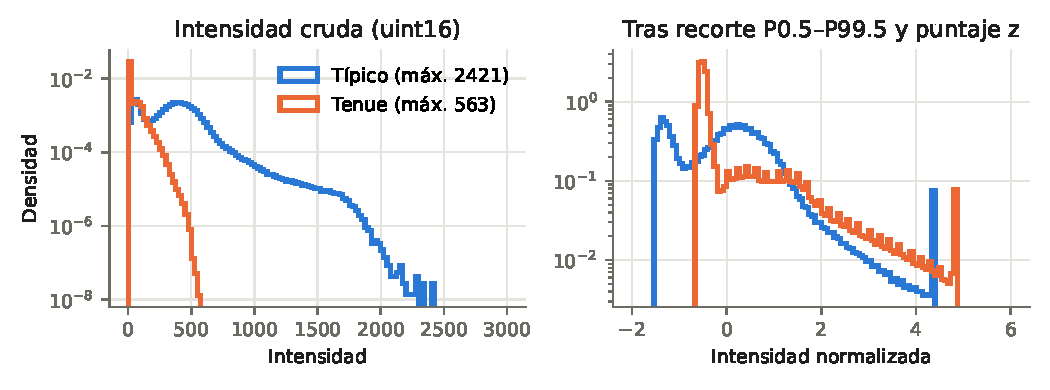
\includegraphics[width=\linewidth]{figs/normalizacion.pdf}
\caption{Histogramas (escala logarítmica) de un volumen típico y del volumen más tenue del conjunto, antes y después de la normalización por volumen. Las barras verticales a la derecha del panel normalizado son los vóxeles acumulados en el percentil 99.5 por el recorte.}
\label{fig:norm}
\end{figure}

\paragraph{Inspección visual de las cajas.} La Figura~\ref{fig:roi} superpone la caja de la anotación sobre un corte positivo y un negativo difícil de un volumen de cada diagnóstico, ya procesado. Confirma tres cosas: \code{roiX} corresponde a la columna y \code{roiY} a la fila (los ejes no están intercambiados), el padding inferior no desplaza las cajas, y la caja abarca la escotadura intercondílea donde se ubica el LCA. También ilustra la limitación señalada en la fase 1: la caja es amplia e incluye parte de los cóndilos, en lugar de ajustarse al ligamento. Los negativos difíciles (a dos cortes de distancia) son visualmente muy parecidos a los positivos, lo que justifica muestrearlos preferentemente.

Para cumplir el criterio de la fase 1 (revisar al menos 30 ejemplos), se inspeccionó además una muestra aleatoria de 30 volúmenes, 10 por diagnóstico, escogida con semilla fija, mostrando el corte positivo central de cada uno (Figura~\ref{fig:inspeccion}). En los 30 casos la caja se ubica sobre la escotadura intercondílea, entre la cara posterior del cóndilo femoral y la meseta tibial, y no se encontró ninguna caja desplazada fuera de la articulación ni con los ejes intercambiados. En todos los casos la caja es sistemáticamente más amplia que el ligamento: incluye parte del cóndilo femoral y de la meseta tibial. Esto confirma, sobre una muestra mayor, que el objetivo es una región de interés amplia y no una caja ajustada. Esta inspección no es una validación clínica, porque no la hizo un especialista, y así debe interpretarse.


\begin{figure}[!htbp]
\centering
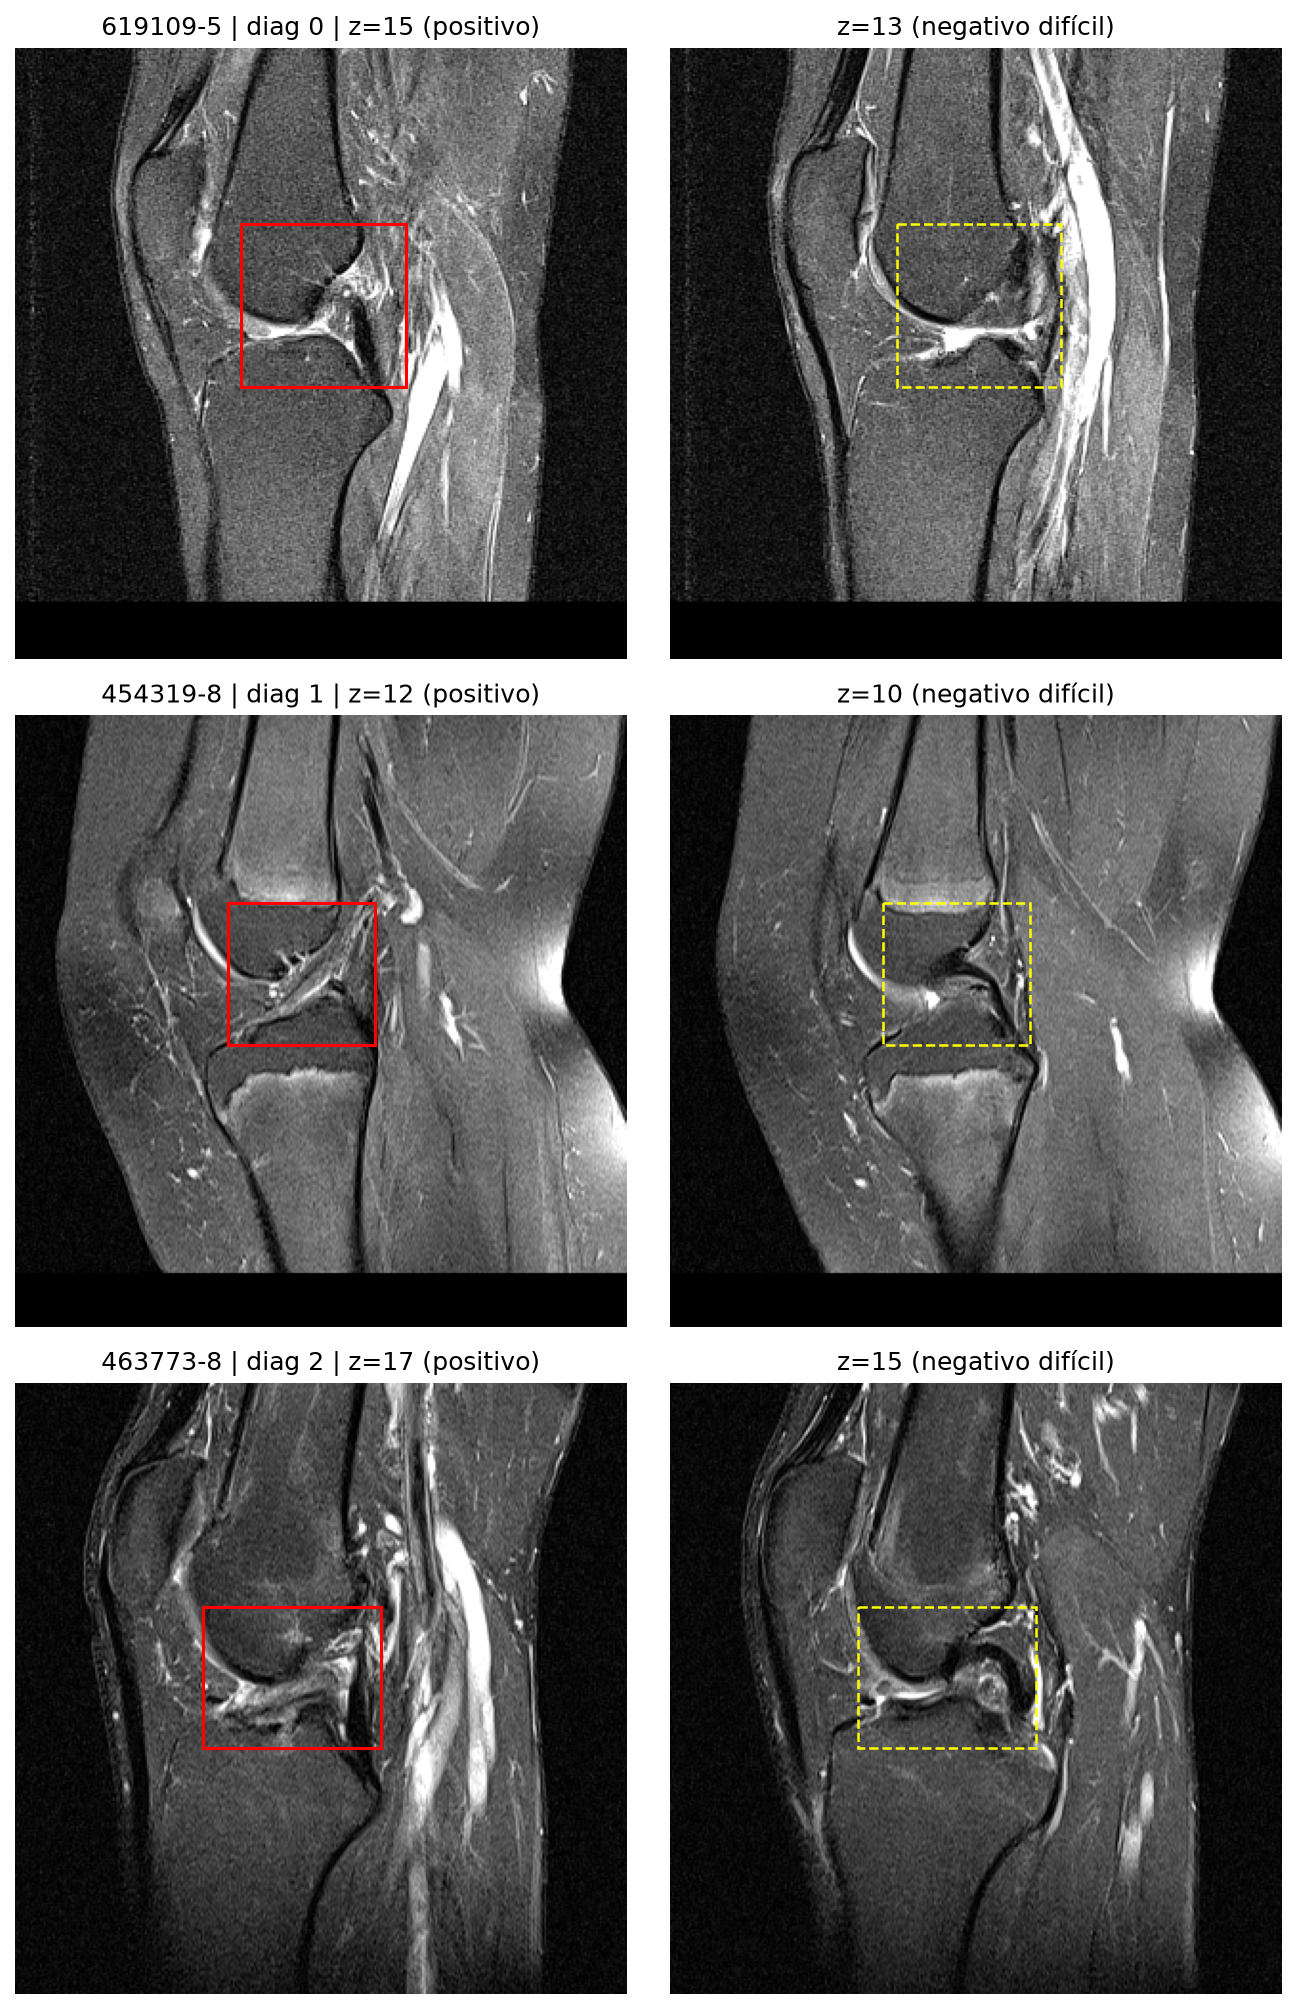
\includegraphics[width=0.46\linewidth]{../figs/roi_check.png}
\caption{Caja anotada sobre volúmenes procesados, uno por diagnóstico (0 sano, 1 parcial, 2 roto). Izquierda: corte positivo. Derecha: negativo difícil a dos cortes de la caja. La banda negra inferior en las dos primeras filas es el padding hasta $320\times320$.}
\label{fig:roi}
\end{figure}

\begin{figure}[!htbp]
\centering
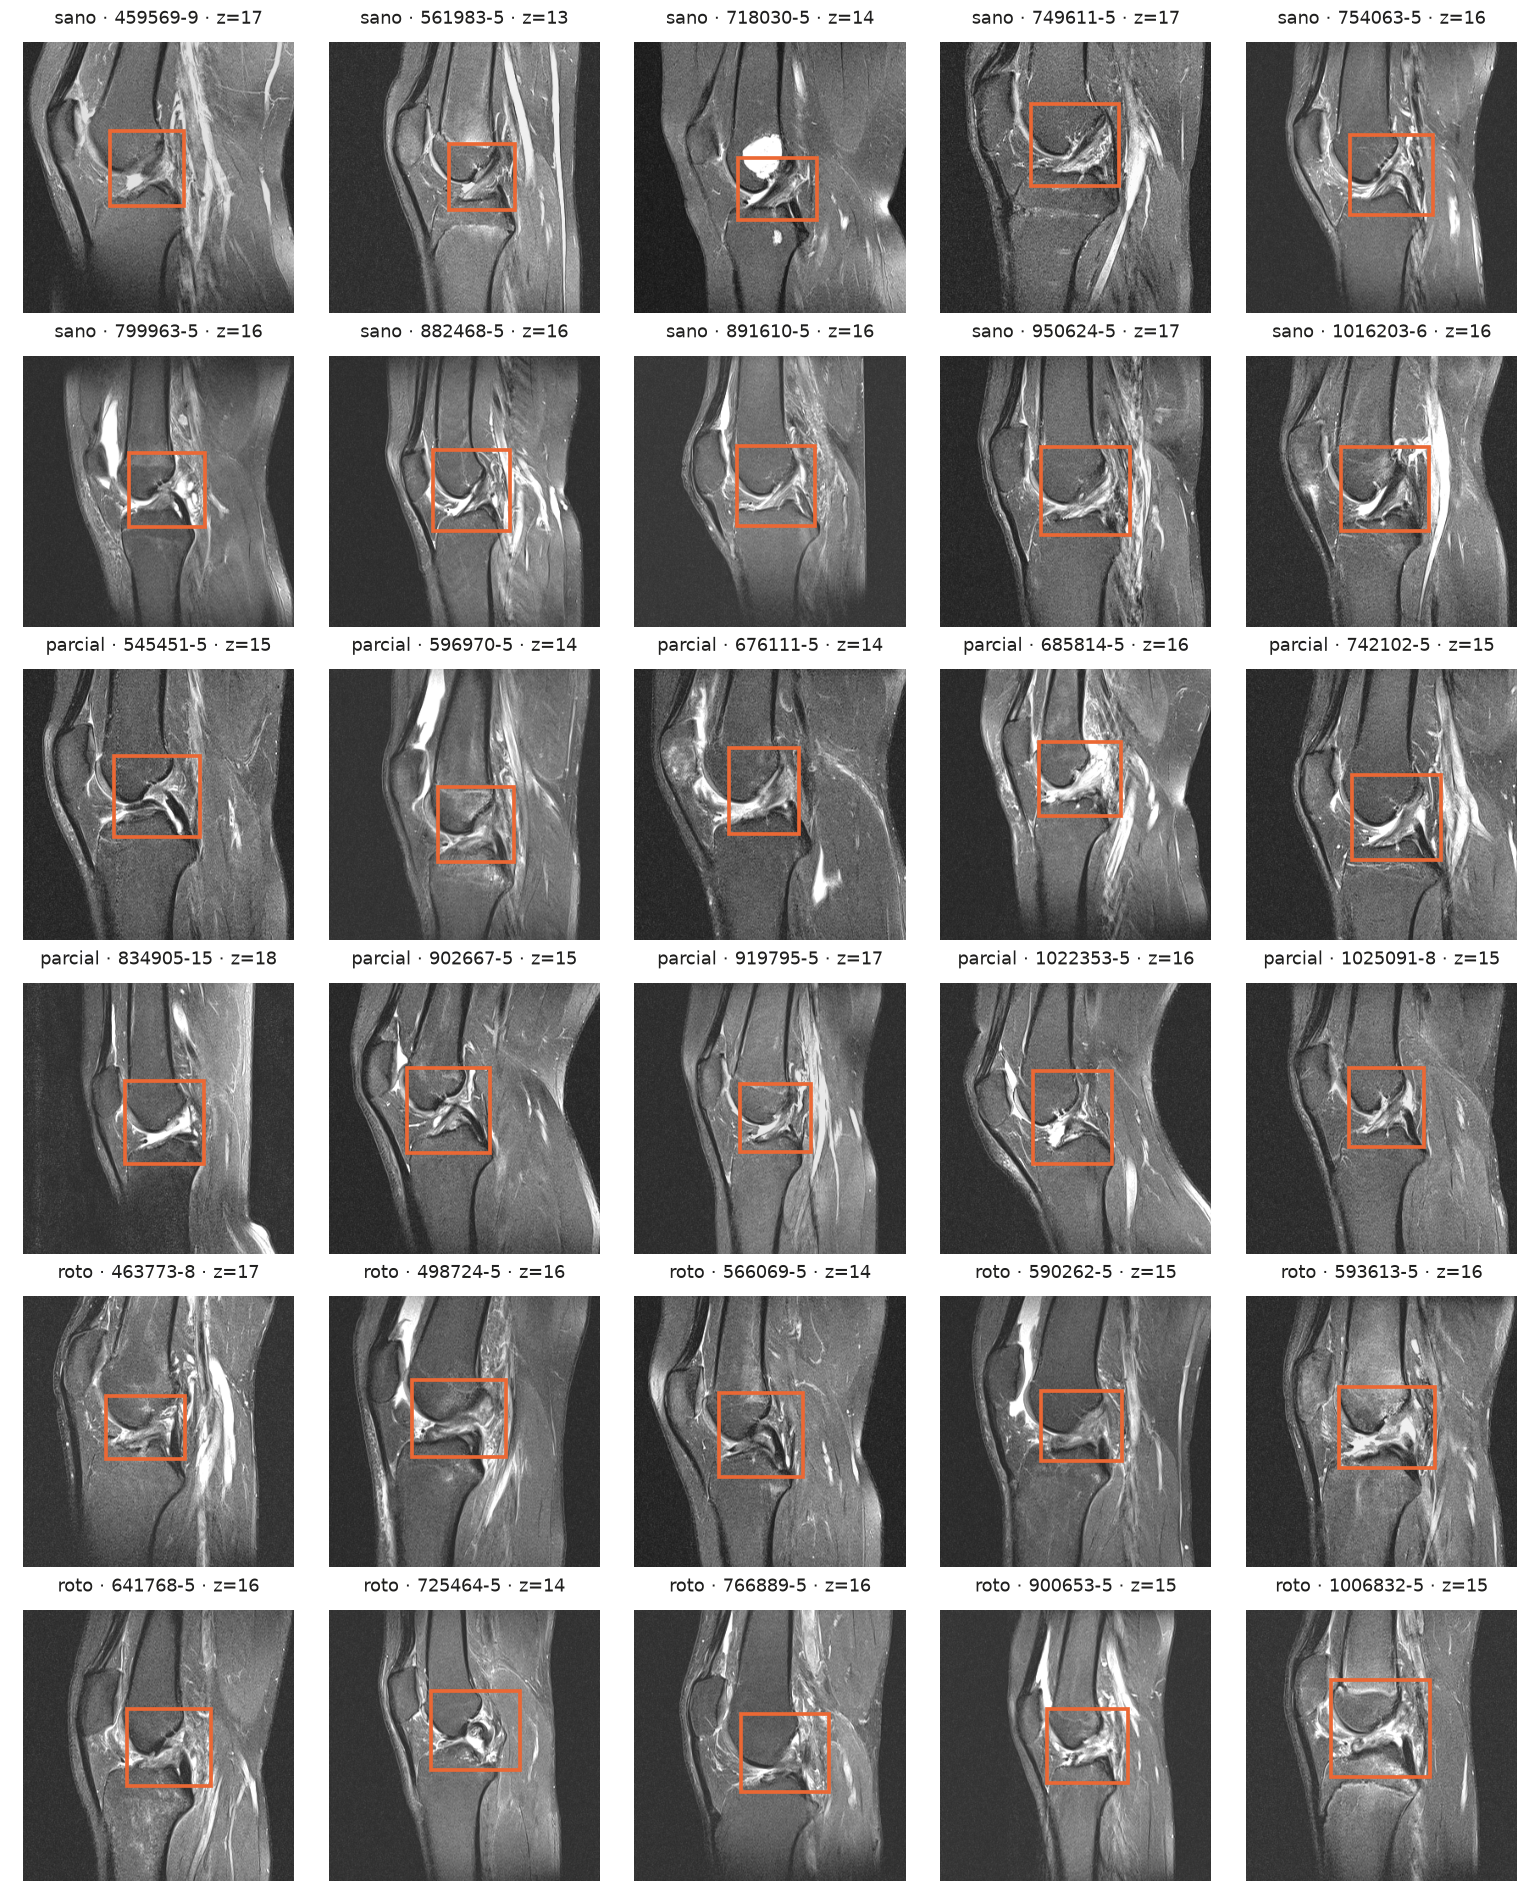
\includegraphics[width=0.92\linewidth]{figs/inspeccion_30.png}
\caption{Inspección visual de 30 volúmenes procesados (10 por diagnóstico, muestra aleatoria con semilla 0): corte positivo central de cada volumen con su caja anotada.}
\label{fig:inspeccion}
\end{figure}

\subsection{Partición}

La Tabla~\ref{tab:splits} muestra la partición resultante. Todas las particiones tienen entre 152 y 153 volúmenes, y la mayor desviación de proporción respecto del total es de \textbf{0.54 puntos porcentuales} (en \code{fold\_3}, que tiene 10 roturas en lugar de 9). Ninguna partición se aleja del ideal en más de un paciente por clase, lo cual es prácticamente el óptimo alcanzable con grupos y solo 55 casos de rotura. Los 7 exámenes con varias series quedaron cada uno completo en una sola partición.

\begin{table}[!htbp]
\centering
\small
\caption{Volúmenes por partición y diagnóstico.}
\label{tab:splits}
\begin{tabular}{lrrrr}
\toprule
Partición & Sano & Parcial & Roto & Total \\
\midrule
\code{fold\_0} & 115 & 29 & 9 & 153 \\
\code{fold\_1} & 115 & 29 & 9 & 153 \\
\code{fold\_2} & 115 & 29 & 9 & 153 \\
\code{fold\_3} & 115 & 28 & 10 & 153 \\
\code{fold\_4} & 115 & 28 & 9 & 152 \\
\code{test}    & 115 & 29 & 9 & 153 \\
\midrule
Total & 690 & 172 & 55 & 917 \\
\bottomrule
\end{tabular}
\end{table}

\subsection{Índice de cortes y desbalance}

El índice contiene \textbf{28\,359 cortes}, de los cuales 3\,081 (10.86\,\%) contienen el LCA (Tabla~\ref{tab:slices}). La proporción de positivos es muy estable entre particiones (10.67\,\% a 11.15\,\%), y cada partición tiene entre 29 y 34 cortes positivos de volúmenes con rotura. El cociente de negativos a positivos en el entrenamiento de cada pliegue varía apenas entre 8.22 y 8.29, de modo que el \code{pos\_weight} será prácticamente el mismo en toda la validación cruzada, aunque se recalcule en cada pliegue como se estableció.

\begin{table}[!htbp]
\centering
\small
\caption{Cortes por partición. ``Roto (+)'' cuenta los cortes positivos de volúmenes con rotura completa.}
\label{tab:slices}
\begin{tabular}{lrrrrr}
\toprule
Partición & Negativos & Positivos & Total & \% positivos & Roto (+) \\
\midrule
\code{fold\_0} & 4\,230 & 505 & 4\,735 & 10.67 & 29 \\
\code{fold\_1} & 4\,225 & 514 & 4\,739 & 10.85 & 30 \\
\code{fold\_2} & 4\,199 & 519 & 4\,718 & 11.00 & 32 \\
\code{fold\_3} & 4\,228 & 513 & 4\,741 & 10.82 & 34 \\
\code{fold\_4} & 4\,229 & 507 & 4\,736 & 10.71 & 30 \\
\code{test}    & 4\,167 & 523 & 4\,690 & 11.15 & 31 \\
\midrule
Total & 25\,278 & 3\,081 & 28\,359 & 10.86 & 186 \\
\bottomrule
\end{tabular}
\end{table}

Dos observaciones adicionales informan la fase 3:

\begin{itemize}[leftmargin=*]
  \item \textbf{La caja abarca en promedio 3.4 cortes en las tres clases} (2\,315/690, 580/172 y 186/55 dan 3.36--3.38). La rotura no cambia la extensión de la anotación en $z$; lo que cambia es la apariencia del ligamento dentro de ella. Por eso el reto de la clase minoritaria es de apariencia y no de geometría.
  \item \textbf{Hay 3\,668 negativos difíciles} ($\code{dist\_to\_roi}\le 2$), el 14.5\,\% de los negativos. Todos los volúmenes tienen al menos seis cortes de margen a cada lado de la caja, así que siempre existen negativos difíciles y fáciles para muestrear.
\end{itemize}

\noindent En el conjunto de desarrollo (764 volúmenes: 575 sanos, 143 parciales, 46 rotos), los pesos de sobremuestreo moderado resultan 1 : 2.0 : 3.5, frente a 1 : 4.0 : 12.5 con peso inverso completo. Esto cuantifica por qué se prefirió la versión moderada.

\subsection{Seguimiento de la tabla de riesgos de la fase 1}

La Tabla~\ref{tab:riesgos} contrasta los riesgos de la fase 1 que correspondían a esta fase con su criterio verificable y el resultado obtenido.

\begin{table}[!htbp]
\centering
\small
\caption{Estado de los riesgos de la fase 1 al cierre de la fase 2.}
\label{tab:riesgos}
\begin{tabular}{p{3.4cm}p{4.6cm}p{6.2cm}}
\toprule
Riesgo (fase 1) & Criterio Q & Resultado \\
\midrule
19.7\,\% de volúmenes faltantes & 0 registros usados sin archivo verificado & \textbf{Resuelto}: descarga completa desde Zenodo, 917/917 verificados; la verificación quedó automatizada en la puerta de calidad. \\
Desbalance sesga los splits & Proporciones por partición a $\pm$2 p.p. del total & \textbf{Cumplido}: desviación máxima de 0.54 p.p., verificada en código. \\
Fuga entre splits & Intersección vacía de \code{examId} & \textbf{Cumplido}: verificado en código; el pipeline se detiene si falla. \\
Objeto pequeño & IoU de validación $\geq$ línea base & \textbf{Mitigado en diseño}: se adoptó la contingencia prevista (representación 2.5D); el criterio se medirá en la fase 3. \\
Caja amplia, no ajustada & Revisar visualmente $\geq$30 ejemplos & \textbf{Cumplido}: 30 volúmenes inspeccionados (10 por clase); todas las cajas sobre la escotadura intercondílea y sistemáticamente más amplias que el ligamento (limitación confirmada, no corregible). \\
\bottomrule
\end{tabular}
\end{table}

\subsection{Limitaciones}

\begin{itemize}[leftmargin=*]
  \item \textbf{Sin identificador de paciente.} La agrupación por \code{examId} es la mejor disponible, pero una misma persona podría tener dos exámenes distintos (ambas rodillas o un control posterior). Esta fuente residual de fuga no puede verificarse con los datos.
  \item \textbf{Pocas roturas en prueba.} Con 9 volúmenes con rotura en prueba, cada uno pesa alrededor del 11\,\% del IoU de esa clase; su estimación tendrá una incertidumbre alta y así deberá reportarse.
  \item \textbf{Caja amplia.} La anotación no es una caja mínima alrededor del ligamento; el IoU medirá el acuerdo con esa anotación y no con la anatomía exacta.
  \item \textbf{Un único centro y equipo.} Nada en esta fase mitiga el sesgo de dominio identificado en la fase 1.
  \item \textbf{Licencia.} KneeMRI se distribuye con licencia CC BY-NC-ND 4.0, que permite el uso académico no comercial; los datos procesados no se redistribuyen.
\end{itemize}

% =========================================================================
\section{Avance y revisión del plan}\label{sec:plan}
% =========================================================================

El plan de la fase 1 situaba la preparación de datos entre las semanas 5 y 9, con cierre el \textbf{6 de octubre}, según la carta al estudiante. Posteriormente, la fecha de entrega de este documento se trasladó al 16 de octubre, así que el entregable se presenta \textbf{a tiempo respecto al calendario vigente del curso}. Medido contra el plan propio, sin embargo, la situación es otra: respecto al plan de la fase 1, \textbf{el proyecto va atrasado aproximadamente diez días}, y el cambio de fecha del curso absorbió ese atraso sin eliminarlo. Las causas principales fueron:

\begin{enumerate}[leftmargin=*]
  \item El descubrimiento de que faltaba el 20\,\% de los volúmenes, que obligó a obtener y verificar una segunda fuente antes de poder particionar.
  \item Varias iteraciones de arquitectura (rutas dependientes del directorio de trabajo, funciones que leían configuración o reconstruían el manifiesto), que se corrigieron antes de avanzar porque afectaban directamente la reproducibilidad.
  \item La decisión entre modelado clásico y aprendizaje profundo, de la cual dependían las transformaciones, que se tomó a mitad de la fase.
\end{enumerate}

\noindent La Tabla~\ref{tab:avance} resume el estado de lo comprometido para esta fase. Todo quedó completo, incluidos tres elementos (pruebas, README e inspección de 30 cajas) que se cerraron el mismo día de la entrega.

\begin{table}[!htbp]
\centering
\small
\caption{Estado de los entregables de la fase 2 comprometidos en el plan.}
\label{tab:avance}
\begin{tabular}{p{7.2cm}p{7.0cm}}
\toprule
Compromiso & Estado \\
\midrule
Verificar la disponibilidad real de archivos & Completo (917/917, automatizado) \\
Splits estratificados y agrupados por examen & Completo y verificado (\code{splits.csv}) \\
Normalizar volúmenes de profundidad variable & Completo, con cambio justificado: no se remuestrea la profundidad (representación 2.5D) \\
Decidir la representación (3D frente a 2.5D) & Completo: 2.5D \\
Pipeline documentado y reproducible & Completo: un comando, configuración en un solo archivo, hashes verificados \\
Pruebas automatizadas (\code{pytest}) & Completo: 31 pruebas, todas pasan \\
README con instrucciones de reconstrucción & Completo (\code{README.md}) \\
Inspección visual de $\geq$30 cajas & Completo (30 de 30, Figura~\ref{fig:inspeccion}) \\
\bottomrule
\end{tabular}
\end{table}

\paragraph{Consecuencias para el resto del plan.} Si se mantiene el 27 de octubre como fecha de las fases 3 (modelado) y 4 (evaluación), quedan once días para instalar PyTorch, implementar el cargador 2.5D con la estrategia de desbalance, entrenar y evaluar, en lugar de las tres semanas que preveía el plan. Es un plazo ajustado. Para absorber el atraso sin sacrificar la calidad se propone:

\begin{itemize}[leftmargin=*]
  \item Comenzar con el modelo más simple que cumple el planteamiento: un único \emph{backbone} preentrenado con las dos cabezas descritas, evaluado primero contra la línea base (IoU 0.391) antes de cualquier optimización de hiperparámetros.
  \item Reducir, si es necesario, la búsqueda de hiperparámetros de la fase 3 a pocos ensayos, sin reducir la validación cruzada ni la evaluación por clase.
  \item Reutilizar directamente lo construido en esta fase: \code{splits.csv} define los pliegues, \code{slices.csv} contiene todo lo necesario para el muestreo, y las pruebas unitarias protegen el código de datos frente a cambios durante el modelado.
\end{itemize}

\noindent El proceso es iterativo: si la fase 3 muestra que la representación 2.5D no supera la línea base, se volverá a esta fase para reconsiderar la representación, por ejemplo con un recorte alrededor de la región típica del LCA. El pipeline permite hacerlo cambiando la configuración y volviendo a ejecutar un comando.

% =========================================================================
\section{Conclusiones}\label{sec:conclusiones}
% =========================================================================

Esta fase convirtió el conjunto KneeMRI en datos listos para entrenar un modelo de localización del LCA mediante un pipeline automatizado, verificable y reproducible. La pregunta que guió cada decisión fue cómo saber que la tarea quedó bien hecha, y la respuesta fue convertir los criterios de calidad de la fase 1 en código que detiene el proceso cuando no se cumplen.

Los resultados más importantes son tres. Primero, el problema de datos faltantes heredado de la fase 1 quedó resuelto y verificado: el proyecto trabaja con los 917 volúmenes, y la puerta de calidad confirmó con los datos que las etiquetas, las cajas y las intensidades son consistentes. Segundo, el riesgo de fuga, el más grave de esta fase, quedó controlado por construcción: la partición agrupada y estratificada se hace antes de cualquier transformación, se congela en un archivo y su verificación es parte del pipeline; además, todas las transformaciones son por volumen y no aprenden de otros datos. Tercero, la elección de una representación 2.5D, junto con el índice de cortes, deja preparada una estrategia concreta y cuantificada para los dos desbalances del problema, que se aplicará en la fase 3 solo sobre los pliegues de entrenamiento.

Persisten limitaciones que no dependen de esta fase: la ausencia de un identificador de paciente, la amplitud de la caja anotada, el reducido número de roturas en prueba y el origen de un único centro. Todas quedan documentadas para matizar la interpretación de los resultados futuros. Finalmente, el entregable llega a tiempo según el calendario vigente del curso, pero el proyecto va unos diez días atrás respecto a su propio plan, y ese atraso reduce el tiempo disponible para el modelado. El atraso es real, pero la base construida en esta fase reduce el riesgo de las siguientes. El pipeline está probado, documentado y verificado, de modo que el modelado podrá concentrarse en el modelo, porque los datos ya no son una fuente de incertidumbre.

\clearpage
\bibliographystyle{ieeetr}
\bibliography{referencias}

\end{document}
